\chapter[Metodologia]{Metodologia} \label{c2}

  A implementação do Pierluigi utilizou a metodologia ágil \textit{Extreme Programming} (XP) como ciclo de vida de desenvolvimento, dado o escopo, o nível de definição dos requisitos e o tamanho da equipe. A XP é um ciclo de vida de desenvolvimento voltado para projetos com equipes pequenas, sistemas orientados a objeto e com desenvolvimento incremental, segundo \citeonline{vinicius}, sendo dividido em iterações que evoluem a aplicação de forma incremental. Primeiramente foi definido o escopo e as ferramentas a serem utilizadas. Então houve o desenvolvimento do protótipo e, por fim, o desenvolvimento da solução planejada.

  \section[Ferramentas Utilizadas]{Ferramentas Utilizadas}

    Antes do início da implementação da solução, foram escolhidas as ferramentas a serem utilizadas no projeto, de acordo com os requisitos levantados. Durante o desenvolvimento, essas foram as ferramentas utilizadas:

  \begin{enumerate}
    \item GitHub\footnotemark \footnotetext{\url{https://github.com/}}: plataforma para hospedagem de código-fonte que utiliza o Git como sistema de controle de versão. Utilizado para o armazenamento do código da solução pelo seu caráter aberto e gratuito;
    \item C++\footnotemark \footnotetext{\url{http://www.cplusplus.com/}}, linguagem de programação compilada multiparadigma. Utilizada como linguagem de implementação principal pelo suporte à programação orientada a objetos e bibliotecas de leitura de arquivos e testes;
    \item Ruby On Rails\footnotemark \footnotetext{\url{https://rubyonrails.org/}}, \textit{framework} para aplicações \textit{web}. Utilizado para desenvolvimento de uma camada \textit{front-end} para a aplicação;
    \item Lilypond\footnotemark \footnotetext{\url{http://lilypond.org/}}, formato de escrita musical baseado em TeX. Utilizado para representação da melodia por ter um formato padronizado e menos verboso se comparado a outras opções como o MusicXML. Além disso, seu pacote para Linux conta com programas como \lstinline{midi2ly} e \lstinline{musicxml2ly}, que permite converter músicas de formatos populares para o formato \lstinline{.ly} padrão do Lilypond;
    \item MuseScore\footnotemark \footnotetext{\url{https://musescore.com/}}, editor de partituras. Utilizado para criação e edição de partitura pelo fato da equipe ter domínio sobre a ferramenta e ser compatível com Linux e Windows, ao contrário de alternativas similares como o Encore.
  \end{enumerate}

  \section[Ciclo de Vida de Desenvolvimento]{Ciclo de Vida de Desenvolvimento}

    O ciclo de vida de desenvolvimento contou com três fases bem definidas. Primeiramente foram levantados os requisitos e então escolhidas as ferramentas a serem utilizadas. Após isso, foi desenvolvido um protótipo focado em contrapontos de primeira espécie. Os resultados do protótipo guiaram o desenvolvimento posterior, que foi focado na composição algorítmica de contrapontos palestrinianos de até quarta espécie e no módulo de construção de MIDI\footnotemark \footnotetext{\textit{Musical Instrument Digital Interface} - Interface Digital de Instrumentos Musicais}.

  \subsection[Requisitos]{Requisitos} \label{sssec:req}

    O escopo inicial era de um \textit{software} capaz de ler uma melodia monofônica e gerar contrapontos palestrinianos de até quarta espécie para ela no formato Lilypond. Veja um fluxograma simplificado da aplicação na Figura \ref{fluxograma}.

    \begin{figure}[htb]
      \centering
      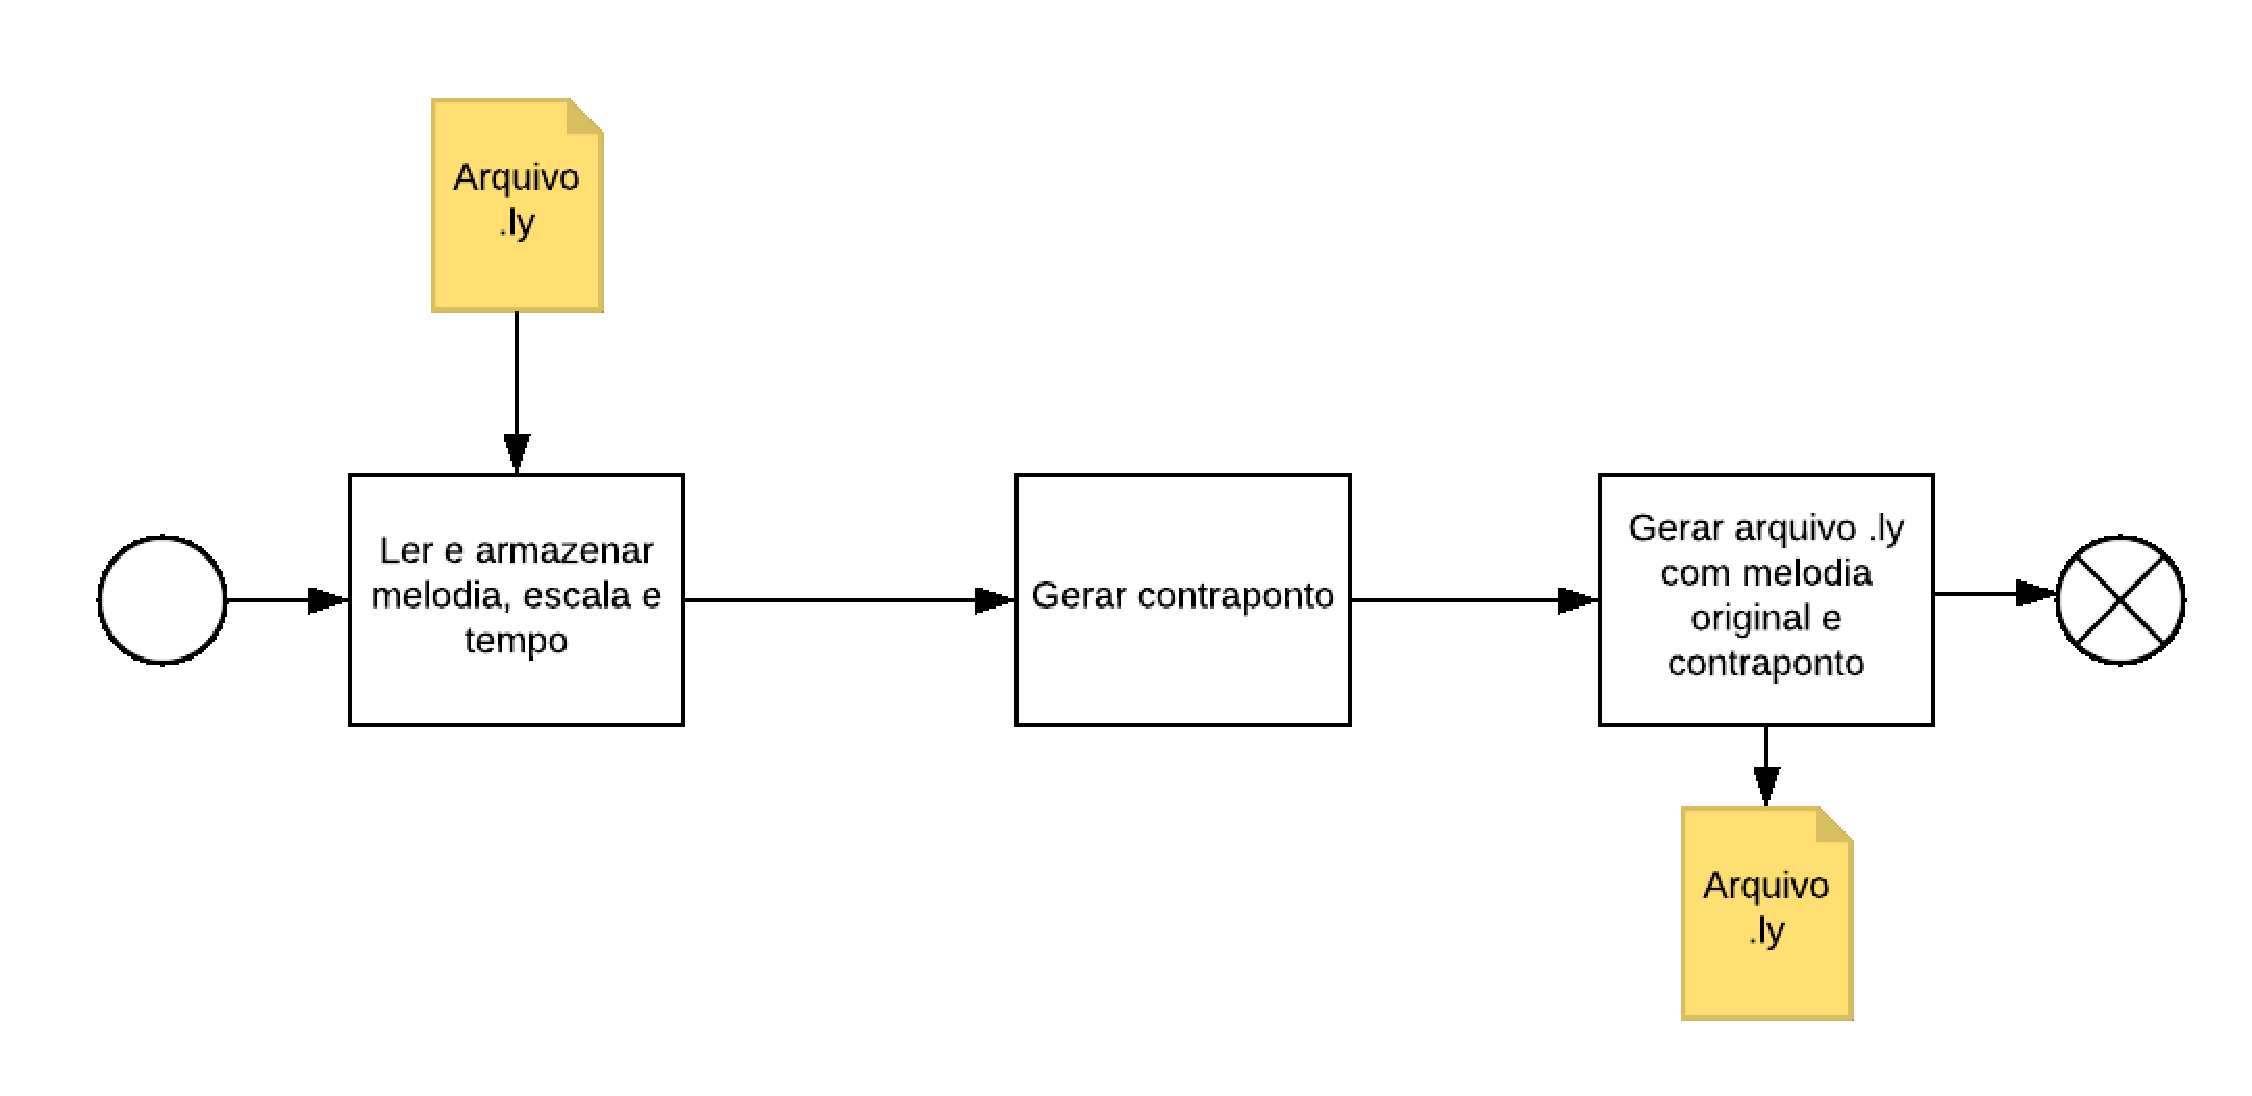
\includegraphics[scale=0.85]{figuras/fluxograma.eps}
      \caption{Fluxograma simplificado da aplicação}
      \label{fluxograma}
    \end{figure}


    Após o estudo da teoria musical necessária para a construção de contrapontos, foram definidos os seguintes módulos a serem desenvolvidos:

    \begin{enumerate}
      \item módulo de notas musicais;
      \item módulo de intervalos;
      \item módulo de escalas;
      \item módulo de contrapontos de primeira espécie;
      \item módulo de contrapontos de segunda espécie;
      \item módulo de contrapontos de terceira espécie;
      \item módulo de contrapontos de quarta espécie;
      \item módulo de construção do MIDI.
    \end{enumerate}

    \subsubsection[Módulo de Notas Musicais]{Módulo de Notas Musicais}

      Este módulo é responsável pela leitura e armazenamento das notas de uma melodia. Ele conta com as seguintes capacidades: armazenamento do atributos de uma nota, \textit{parser} de uma nota em formato Lilypond e armazenamento de uma melodia completa. O armazenamento de uma nota inclui estes atributos: a figura musical que representa a duração, o tempo absoluto da nota, os acidentes aplicados a ela, a oitava em que ela está inserida, seu número MIDI e seu número em relação a notas sem contar acidentes. Além disso, essa parte deve ser capaz de devolver notas enarmônicas a uma nota -- notas com nomenclatura diferente, mas som e número de semitons (em relação a uma nota qualquer) iguais, como C\sh{}  e D\fl.

      O \textit{parser} de uma nota deve ser feito a partir de um arquivo Lilypond e armazenado na estrutura responsável pelo armazenamento de notas já citada. Além disso, ele deve ser capaz de retornar uma nota armazenada no mesmo formato lido.

      O arquivo lido deve ter as seguintes caraterísticas para que funcione corretamente na solução:

      \begin{enumerate}
        \item Deve ter apenas uma melodia e ela deve ser monofônica. Se possuir mais de uma melodia, apenas a primeira será considerada para a geração do contraponto.
        \item A melodia principal deve possuir escala e ritmo definidos explicitamente.
        \item A nota mais curta da melodia principal deve ser uma colcheia sem pontos de aumento.
      \end{enumerate}

      O armazenamento da melodia completa deve ser capaz de armazenar as notas de uma melodia preservando sua ordem, além de armazenar o tempo dos compassos e a escala da música.

    \subsubsection[Módulo de Intervalos]{Módulo de Intervalos}

      O módulo de intervalos deve ser capaz de armazenar intervalos, gerá-los a partir de duas notas ou de uma \textit{string} e de retornar a outra nota dados uma nota e um intervalo. Por exemplo, retornar G\sh5 ao receber C5 e um intervalo de quinta aumentada.

      O armazenamento de intervalos deve possuir os seguintes atributos: classificações quantitativa e qualitativa, número de semitons e se o intervalo é ascendente ou não (considerando a nota recebida como primeira).

      O método de retorno de uma nota, dado uma nota e um intervalo, deve ser capaz de retornar a segunda nota para qualquer intervalo definido, de forma que a distância entre as duas notas seja compatível com a classificação quantitativa e qualitativa do intervalo. Ele também deve ser capaz de indicar se é impossível gerar tal nota e retornar uma nota em uma dada escala previamente definida, quando necessário.

    \subsubsection[Módulo de Escalas]{Módulo de Escalas}

      O módulo de escalas deve ser capaz de armazenar uma escala e responder se uma nota faz ou não parte dela. O armazenamento da escala deve ser capaz de armazenar quais notas estão presentes nela a partir da primeira nota e do modo (maior ou menor) ou da primeira nota e de um conjunto de intervalos.

      O objeto de uma escala deve ser capaz de receber um objeto de nota e dizer se aquela nota está ou não presente, baseada em seu número de MIDI e sua representação. Por exemplo, a nota B está presente na escala de Dó Maior, mas não a nota C\fl{}, embora elas sejam enarmônicas.

    \subsubsection[Módulos de Contraponto]{Módulo de Contraponto}

      Cada módulo deve ser capaz de gerar um contraponto palestriniano de acordo com as regras definidas pela espécie do contraponto. Eles devem receber uma melodia monofônica e gerar um contraponto daquela espécie de acordo com os parâmetros fornecidos em relação a número de movimentos reversos, consonâncias condicionais paralelas e outros parâmetros relacionados a regras que não sejam exatas.

      Como exemplo, tem-se a regra que se evita, mas não se proíbe, movimentos paralelos, cabendo ao usuário definir o número de movimentos paralelos aceitáveis. Com tais parâmetros, o módulo deve ser capaz de gerar um contraponto aleatório para cada iteração do algoritmo.

      No desenvolvimento desse módulo é usada a DFS por dois motivos. O primeiro é que a DFS chega a uma folha (vértice sem filhos) primeiro, o que é interessante para a solução pois busca-se a primeira solução disponível. O segundo motivo é que a DFS permite que seja utilizado um único vetor, inserindo e retirando no final deste (consequentemente, funcionando de forma análoga a uma pilha), economizando memória e diminuindo o tempo de execução que levaria para fazer cópias do vetor em uma BFS, pois o comportamento análogo a uma fila exigiria isso.

      A DP é utilizada para a geração do contraponto. O estado é caracterizado por uma dada nota em uma dada posição no contraponto com um número específico de movimentos paralelos e terças e sextas paralelas. A transição é definida pela solução da próxima nota no contraponto, partindo da nota atual. O caso-base é definido por quando o algoritmo atinge o final do \textit{cantus firmus}, retornando que aquela solução é válida, já que não foi podada nenhuma vez durante a construção daquela solução.

    \subsubsection[Módulo de Construção do MIDI]{Módulo de Construção do MIDI}

      Segundo \cite{midi}, o MIDI é um padrão de comunicação entre intrumentos musicais digitais amplamente aceito com especificações para \textit{hardware} de comunicação, taxa de transferência de dados e formato de dados transferidos. Os arquivos .mid não são áudios, mas instruções digitais sobre como executar uma peça musical.

      O módulo de construção do MIDI é um módulo que deve automatizar a construção de um MIDI tendo como base o arquivo Lilypond original e o contraponto gerado. Com esses dois, esse módulo deve inserir o contraponto em uma cópia do arquivo original e gerar o MIDI utilizando o pacote do Lilypond para Linux.

  \subsection[Protótipo]{Protótipo}

    O protótipo possui a finalidade de testar o conceito da solução por meio um MVP (produto mínimo viável ou \textit{minimum viable product}). O protótipo proposto possui as seguintes funcionalidades:

    \begin{enumerate}
      \item módulo de notas musicais, incluindo leitura de arquivo Lilypond simplificado e armazenamentos de notas de uma melodia;
      \item módulo de intervalos, incluindo a construção de intervalos a partir de notas ou \textit{strings} padronizadas e retorno de nota ao se receber nota e intervalo;
      \item módulo de escalas, incluindo construção de escalas a partir do modo ou de um conjunto de intervalos;
      \item módulo de contrapontos de primeira espécie implementado utilizando busca completa;
      \item módulo de contrapontos de primeira espécie implementado utilizando programação dinâmica;
      \item módulo de contrapontos de segunda espécie, com leitura de tempo de compasso.
    \end{enumerate}

    O protótipo contém os módulos de notação, intervalos e escalas pois são considerados módulos básicos para a construção de contrapontos.

    O módulo de contrapontos de primeira espécie com algoritmo de busca completa pretende testar se a geração de contrapontos de forma \textit{naive} (a implementação mais simples possível) é correta e computacionalmente viável.

    O módulo de contrapontos de segunda espécie com algoritmo de DP pretende testar se a programação dinâmica efetivamente diminui o tempo de execução do algoritmo e se essa diminuição é relevante o suficiente para justificar o uso desse paradigma.

    O módulo de contrapontos de segunda espécie busca validar a corretude do módulo de primeira espécie uma vez que tenha sido escalado. Dentre as novas dificuldades, há o fato de que há duas notas no contraponto para cada do \textit{cantus firmus}, a posição da nota no compasso possui papel decisivo no algoritmo, invalidando a estratégia de avaliar os intervalos nota a nota e adicionando um estado à DP.

  \subsection[Desenvolvimento]{Desenvolvimento}

    Após a definição dos requisitos e a construção do protótipo, o sistema teve o restante de suas funcionalidades implementadas e testadas. As atividades da fase de desenvolvimento são:

    \begin{enumerate}
      \item testes dos módulos de notação, intervalos e escalas;
      \item testes dos módulos de contraponto de primeira e segunda espécie;
      \item otimização do \textit{parser};
      \item implementação e testes do módulo de contrapontos de terceira espécie;
      \item implementação e testes do módulo de contrapontos de quarta espécie;
      \item implementação e testes do módulo de contrapontos de quinta espécie;
      \item implementação e testes do módulo de construção de MIDI.
    \end{enumerate}

    O desenvolvimento iniciou com testes das funcionalidades implementadas no protótipo. O objetivo é garantir que a solução do protótipo é adequada e completa antes de começar a implementação definitiva, refatorando o código e removendo \textit{bugs} identificados.

    Após isso, houve a otimização do \textit{parser}. O \textit{parser} do potótipo lê apenas um arquivo Lilypond modificado para conter apenas o tempo, a escala e as notas. Foi implementado um \textit{parser} que, ainda que simples, é capaz de ler arquivos Lilypond sem tais modificações.

    Seguindo a otimização do \textit{parser}, houve a implementação e teste dos contrapontos de terceira e quarta espécie. Baseado no código já implementado dos contrapontos de primeira e segunda espécie, eles foram desenvolvidos sequencialmente, já que as novas regras de uma espécie somam-se às regras da espécie anterior.

    Por fim, houve a implementação de um módulo de construção de MIDI com as especificações definidas na Subseção \ref{sssec:req}.

  \section[Atividades]{Atividades}

  O desenvolvimento do sistema teve as seguintes atividades:

  \begin{enumerate}
    \item \label{t1} definição dos requisitos do sistema;
    \item \label{t2} estudo sobre teoria musical, incluindo notação musical, intervalos, escalas e contrapontos;
    \item \label{t3} implementação do protótipo de parser de um arquivo Lilypond;
    \item \label{t4} implementação do módulo de notas musicais;
    \item \label{t5} implementação do módulo de intervalos;
    \item \label{t6} implementação do módulo de escalas;
    \item \label{t7} implementação do protótipo do módulo de contrapontos;
    \item \label{t8} implementação do módulo de contrapontos de primeira espécie utilizando busca completa;
    \item \label{t9} implementação do módulo de contrapontos de primeira espécie utilizando programação dinâmica;
    \item \label{t10} escrita do TCC 1;
    \item \label{t11} implementação do módulo de contrapontos de segunda espécie;
    \item \label{t12} testes do \textit{parser};
    \item \label{t13} testes do módulo de notas musicais;
    \item \label{t14} testes do módulo de intervalos;
    \item \label{t15} testes do módulo de escalas;
    \item \label{t16} testes dos módulos de contrapontos de primeira e segunda espécie;
    \item \label{t17} otimização do \textit{parser};
    \item \label{t18} implementação e testes do módulo de contrapontos de terceira espécie;
    \item \label{t19} implementação e testes do módulo de contrapontos de quarta espécie;
    \item \label{t20} implementação e testes do módulo de construção de MIDI;
    \item \label{t21} escrita do TCC 2.
  \end{enumerate}

%   O cronograma do trabalho está apresentado na Figura \ref{crono}.
%
%   \begin{figure}[htb]
%     \centering
%   \begin{ganttchart}[
%     vgrid,
%     hgrid,
%     bar label font=\Large,
%     bar label text={#1$\rightarrow$},
%     group label font=\color{orange},
%     group label text={#1},
%     bar/.append style={fill=green!50},
%     milestone label font=\color{red},
%     milestone label node/.append style={rotate=0},
%     milestone label text={#1},
%     x unit=1.2cm,
%     y unit title=1.2cm,
%     y unit chart=0.8cm,
%   ]{1}{10}
%     \gantttitle{Cronograma do Trabalho}{10} \\
%     \gantttitlecalendar*[compress calendar,time slot format=isodate]{2018-3-1}{2018-12-10}{year, month} \\
%     \ganttbar{\ref{t1}}{1}{1} \\
%     \ganttbar{\ref{t2}}{1}{2} \\
%     \ganttbar{\ref{t3}}{1}{1} \\
%     \ganttbar{\ref{t4}}{1}{1} \\
%     \ganttbar{\ref{t5}}{2}{2} \\
%     \ganttbar{\ref{t6}}{3}{3} \\
%     \ganttbar{\ref{t7}}{2}{3} \\
%     \ganttbar{\ref{t8}}{2}{2} \\
%     \ganttbar{\ref{t9}}{2}{3} \\
%     \ganttbar{\ref{t10}}{2}{4} \\
%     \ganttbar[bar/.append style={fill=yellow!50}]{\ref{t11}}{4}{5} \\
%     \ganttbar[bar/.append style={fill=red!50}]{\ref{t12}}{5}{6} \\
%     \ganttbar[bar/.append style={fill=red!50}]{\ref{t13}}{5}{6} \\
%     \ganttbar[bar/.append style={fill=red!50}]{\ref{t14}}{5}{6} \\
%     \ganttbar[bar/.append style={fill=red!50}]{\ref{t15}}{5}{6} \\
%     \ganttbar[bar/.append style={fill=red!50}]{\ref{t16}}{5}{6} \\
%     \ganttbar[bar/.append style={fill=red!50}]{\ref{t17}}{6}{6} \\
%     \ganttbar[bar/.append style={fill=red!50}]{\ref{t18}}{6}{7} \\
%     \ganttbar[bar/.append style={fill=red!50}]{\ref{t19}}{7}{8} \\
%     \ganttbar[bar/.append style={fill=red!50}]{\ref{t20}}{8}{9} \\
%     \ganttbar[bar/.append style={fill=red!50}]{\ref{t21}}{9}{10} \\
%     \ganttbar[bar/.append style={fill=red!50}]{\ref{t22}}{8}{10}
%
%   \end{ganttchart}
%   \caption{Cronograma}
%   \label{crono}
%
% \end{figure}
